\section*{Ensayo}

{
    A continuaci\'on se describe una serie de pasos que se llevar\'on a cabo para
    implementar una topolog\'ia de red.
    \renewcommand{\labelitemi}{$\diamond$}
    \begin{itemize}
        \item Se conoci\'o la funcionalidad del cable de consola, cuales son los casos en los que se usa 
        y en que entornos es utilizado. El cable de consola necesita ser conectado a un puerto de serie, pero 
        debido a que las computadoras modernas no tienen este puerto es utilizado un adaptador USB para lograr 
        la comunicaci\'on con el Switch.
        \begin{figure}[h]
            \hspace{1cm}
            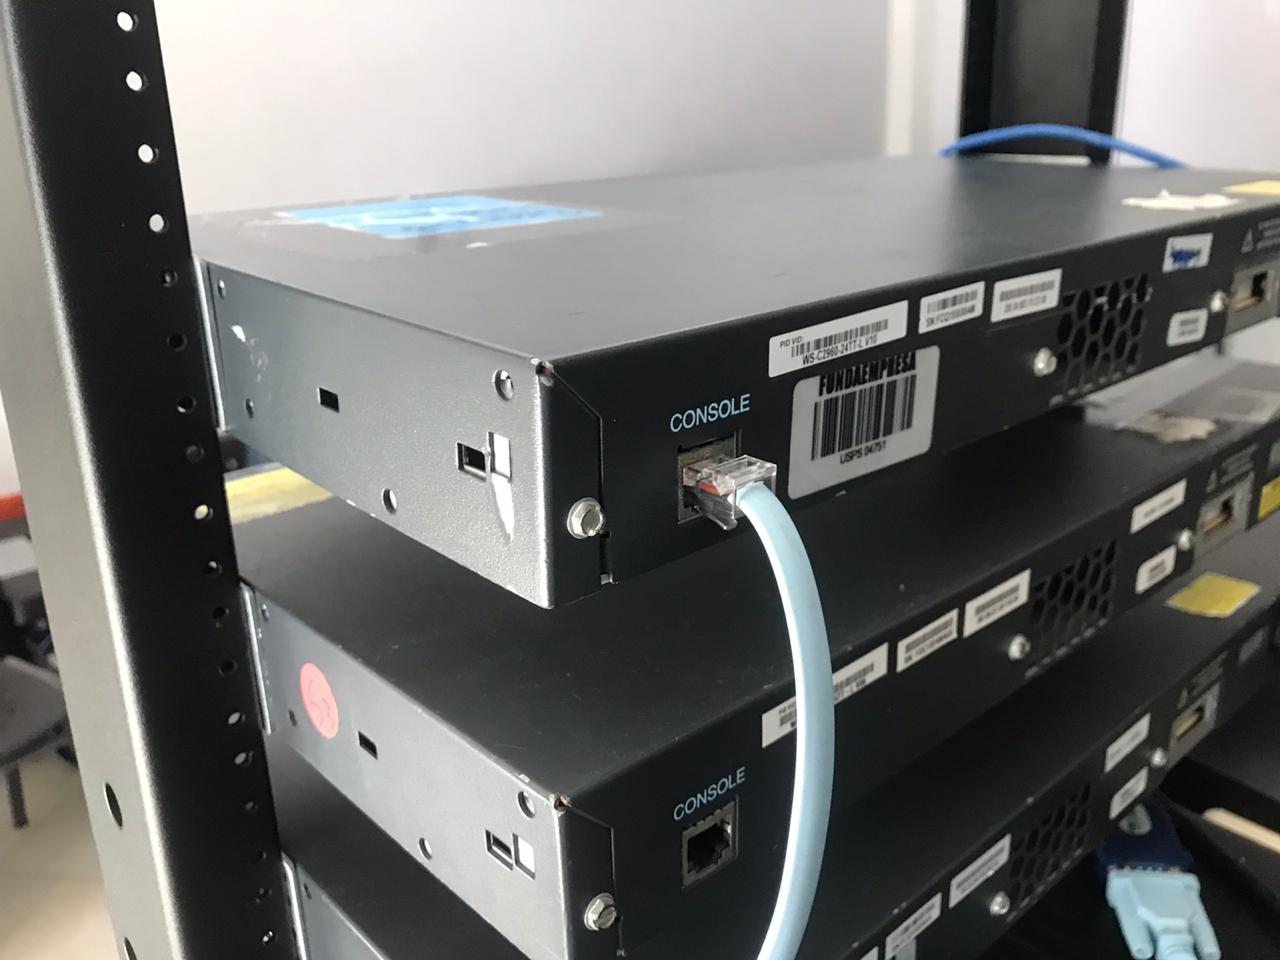
\includegraphics[width=7cm, height=4cm]{imagenes/cable_consola.jpeg}
            \hspace{0.5cm}
            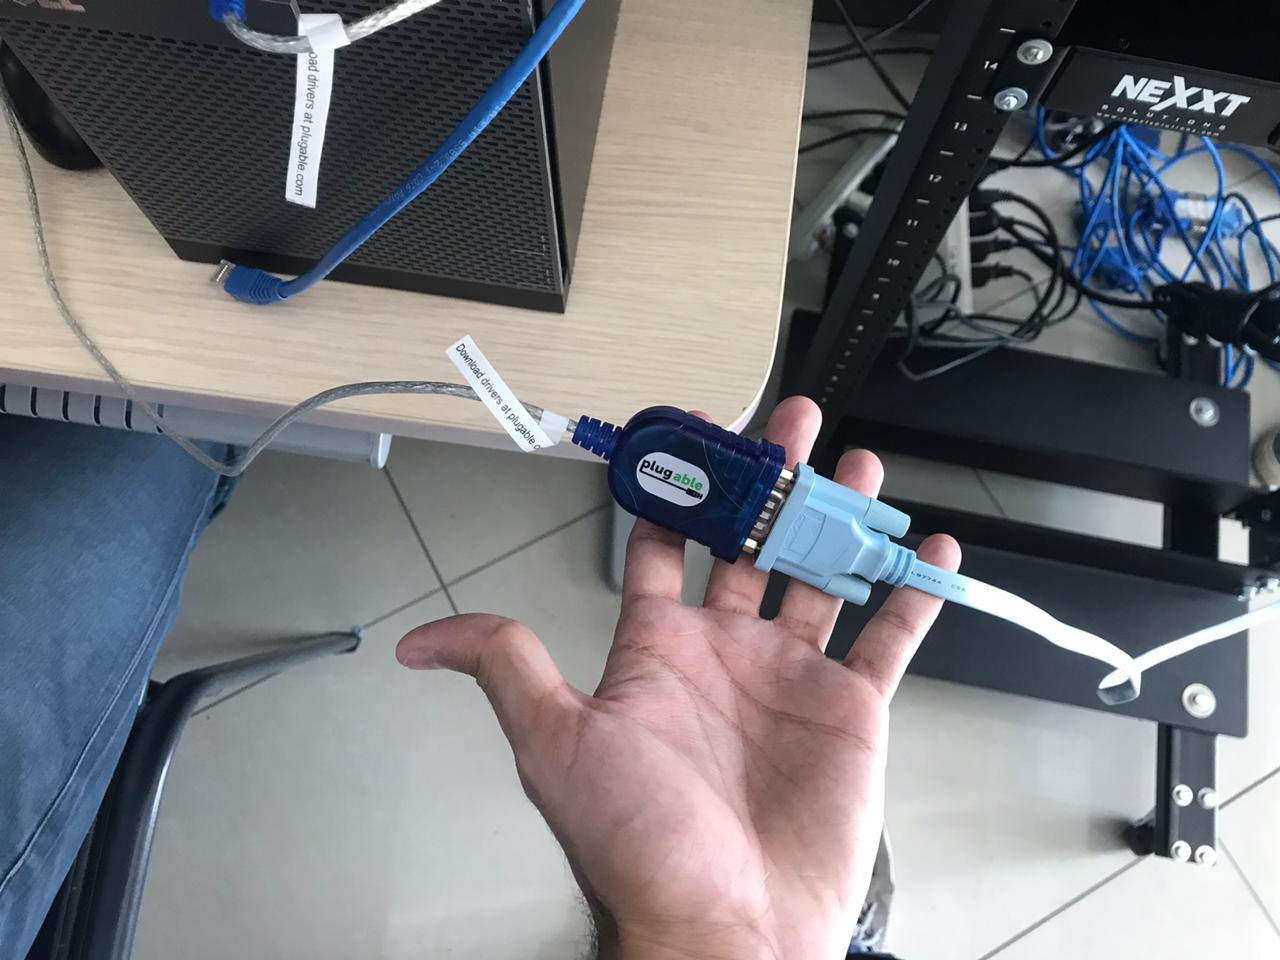
\includegraphics[width=7cm, height=4cm]{imagenes/cable_consola2.jpeg}
        \end{figure}

        \item A trav\'es de la aplicaci\'on PuTTY se estableci\'o la comunicaci\'on necesaria con el Switch.
        Esto abre una sesi\'on de comunicaci\'on serial de 9600 bps, 8 bits de data, sin bit de paridad, 
        1 bit de parada y sin control de flujo.
        
        \item Se ejecutaron los comandos de verificaci\'on y configuraci\'on.
        \begin{figure}[h]
            \hspace{1cm}
            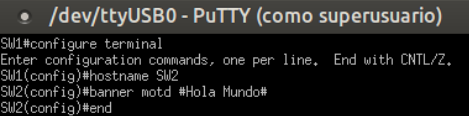
\includegraphics[width=7cm, height=4cm]{./imagenes/terminal_1.png}
            \hspace{0.5cm}
            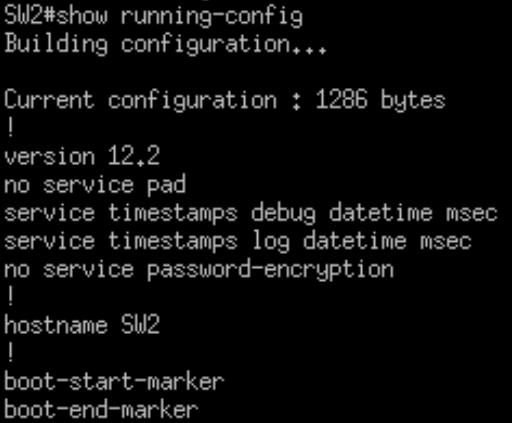
\includegraphics[width=7cm, height=4cm]{./imagenes/terminal_2.png}
        \end{figure}
        
        \newpage %salto a una nueva pagina
        \item Para comprobar que la conexi\'on estaba establecida se ejecut\'o el comando: \textbf{show mac address-table}
        \begin{figure}[h]
            \hspace{4cm}
            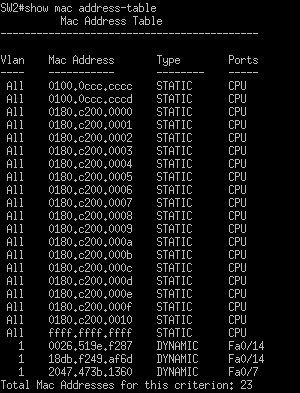
\includegraphics[width=8cm, height=8cm]{./imagenes/terminal_3.png}
        \end{figure}
    \end{itemize}
    
    En la siguiente secci\'on se responden una serie de preguntas de an\'alisis e investigaci\'on.

    \renewcommand{\labelitemi}{$\circ$}
    \begin{itemize}
        \item ?`Fue necesario implementar un router para que dos computadoras puedan comunicarse entre s\'i?
        \begin{itemize}
            \item[] \textit{No fu\'e necesario implementar un router; solo hab\'ia que configurar el switch correctamente y configurar las 
            PC's con las IP's correctas. La conexi\'on necesit\'o de un protocolo.}

            \item[] La funci\'on de un switch es el de transmitir la informaci\'on a los diferentes dispositivos interconectados con la red. 
            Su labor es muy similar al de una central telef\'onica. Cuando uno de los dispositivos env\'ia un mensaje, el conmutador se 
            encarga de leerlo y reenviarlo al equipo que corresponda. De esta manera, se reduce el congestionamiento en la red. 
            Para ello, es necesario una tarjeta de red llamada MAC, la cual llevar\'a el servicio solicitado al equipo de destino, 
            permitiendo as\'i la comunicaci\'on eficiente entre los dispositivos interconectados. \cite{ChTech}
        \end{itemize}
        
        \item ?`Que hace falta para que dos computadoras puedan comunicarse entre s\'i?
        \begin{itemize}
            \item[] \textit{Una vez las dos m\'aquinas est\'an configuradas se necesita de un protocolo que haga posible el env\'io de 
            paquetes de una m\'aquina a otra.}
        \end{itemize}
        
        \newpage
        \item ?`Que es el protocolo ARP y que funci\'on cumple dentro de la comunicaci\'on entre dos computadoras? 
        ?`En que momento la tabla MAC de direcciones de los router y las computadoras cambi\'o? Explique y desarrolle.
        \begin{itemize}
            \item[] \textit{ARP del acr\'onimo Address Resolution Protocol} es un protocolo ejecutado en cas\'i todas las m\'aquinas que
            se conectan a internet. Es una manera simple de comunicaci\'on que se puede reemplazar por los archivos de configuraci\'on.
            El administrador del sistema s\'olo tiene que asignar a cada m\'aquina una direcci\'on IP y decidir respecto a las m\'ascaras
            de subred. ARP se hace cargo del resto. \cite{Tanenbaum}
            
            \item[] \textit{La tabla MAC de direcciones cambi\'o cuando se ejecut\'o el comando ipconfig (ifconfig en Linux) y se ejecuto el
            comando} \textbf{arp -a} \textit{en ambas computadoras. Luego de hacer ping a una m\'aquina, la tabla MAC debi\'o quedar actualizada.}

            \item [] Es posible hacer varias optimizaciones para que ARP trabaje con m\'as eficiencia. Para empezar, una
            vez que una m\'aquina ha ejecutado ARP, guarda el resultado en cach\'e, en caso de que tenga que ponerse
            en contacto con la misma m\'aquina en poco tiempo. La siguiente vez encontrar\'a la asociaci\'on en su propio
            cach\'e, con lo cual se elimina la necesidad de una segunda difusi\'on. En muchos casos, el host 2 necesitar\'a
            devolver una respuesta y se ver\'a forzado tambi\'en a ejecutar el ARP para determinar la direcci\'on Ethernet
            del emisor. \cite{Tanenbaum}
        \end{itemize}
    \end{itemize}
}